\documentclass[tikz,border=3pt]{standalone}
\usepackage[utf8]{inputenc}
\usepackage[T1]{fontenc}
\usepackage{lmodern}
\renewcommand{\familydefault}{\sfdefault}
\usepackage{sansmath}\sansmath
\usepackage{chemfig}
\usepackage{pgfplots}\pgfplotsset{compat=1.18,/pgf/number format/use comma,/pgf/number format/1000 sep={.}}
\usetikzlibrary{arrows.meta,calc,positioning,decorations.pathmorphing,patterns}
% paleta del sitio
\definecolor{nar}{HTML}{E8680C}\definecolor{narc}{HTML}{FFB35C}\definecolor{hielo}{HTML}{FFF3E8}
\definecolor{tinta}{HTML}{1D1D1F}\definecolor{gris}{HTML}{6E6E73}\definecolor{lila}{HTML}{7C5CF0}
\definecolor{azul}{HTML}{2F6FD6}\definecolor{menta}{HTML}{17A673}\definecolor{coral}{HTML}{E8342A}
\begin{document}
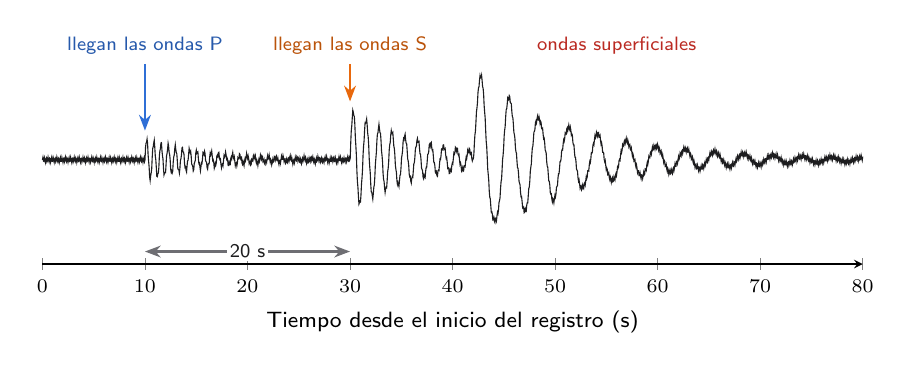
\begin{tikzpicture}[font=\footnotesize,>={Stealth[length=2mm]}]
\begin{axis}[width=12cm,height=4.6cm,xmin=0,xmax=80,ymin=-1.25,ymax=1.6,
  xlabel={Tiempo desde el inicio del registro (s)},ytick=\empty,axis y line=none,axis x line=bottom,
  xtick={0,10,20,30,40,50,60,70,80},tick label style={font=\scriptsize},label style={font=\footnotesize},clip=false]
\addplot[tinta,thin,samples=1600,domain=0:80] {0.03*sin(deg(37*x)) + (x>10)*0.25*exp(-(x-10)/6)*sin(deg(9*(x-10))) + (x>30)*0.6*exp(-(x-30)/7)*sin(deg(5*(x-30))) + (x>42)*1.0*exp(-(x-42)/10)*sin(deg(2.2*(x-42)))};
\draw[->,azul,thick] (axis cs:10,1.15) -- (axis cs:10,0.35);
\node[font=\scriptsize,text=azul!80!black,anchor=south] at (axis cs:10,1.15) {llegan las ondas P};
\draw[->,nar,thick] (axis cs:30,1.15) -- (axis cs:30,0.7);
\node[font=\scriptsize,text=nar!80!black,anchor=south] at (axis cs:30,1.15) {llegan las ondas S};
\node[font=\scriptsize,text=coral!80!black,anchor=south] at (axis cs:56,1.15) {ondas superficiales};
\draw[<->,gris,thick] (axis cs:10,-1.1) -- (axis cs:30,-1.1) node[midway,fill=white,font=\scriptsize,text=tinta,inner sep=1pt] {20 s};
\end{axis}
\end{tikzpicture}
\end{document}
